\begin{figure}[p]
\centering

\includegraphics[width=5.5in]{figs/v9_blocks_Qwen-Qwen3-0.6B_legend.pdf}\\[1pt]
\begin{subfigure}[t]{2.7in}\centering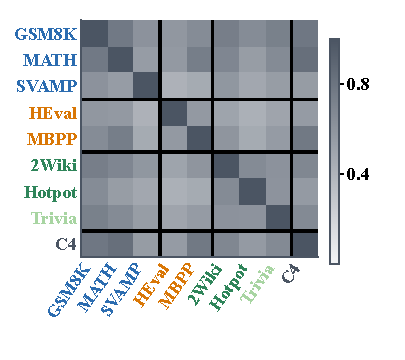
\includegraphics[width=\linewidth]{figs/v9_blocks_Qwen-Qwen3-0.6B_a.pdf}\subcaption{Raw Fisher cosine}\end{subfigure}
\hfill
\begin{subfigure}[t]{2.7in}\centering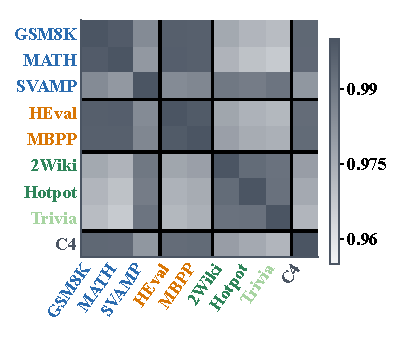
\includegraphics[width=\linewidth]{figs/v9_blocks_Qwen-Qwen3-0.6B_b.pdf}\subcaption{Log-Fisher cosine}\end{subfigure}
\\[3pt]
\begin{subfigure}[t]{2.7in}\centering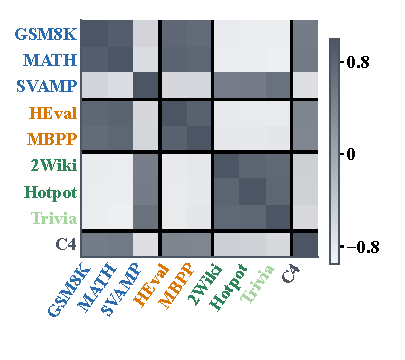
\includegraphics[width=\linewidth]{figs/v9_blocks_Qwen-Qwen3-0.6B_c.pdf}\subcaption{Residual log-Fisher cosine}\end{subfigure}
\hfill
\begin{subfigure}[t]{2.7in}\centering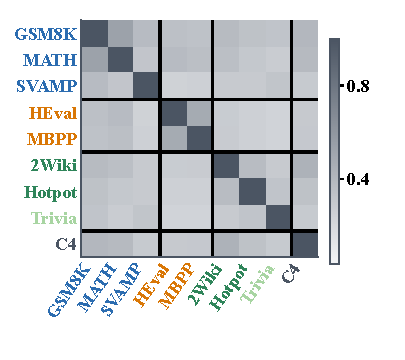
\includegraphics[width=\linewidth]{figs/v9_blocks_Qwen-Qwen3-0.6B_d.pdf}\subcaption{Top-0.1\% Jaccard}\end{subfigure}
\caption{Capability regions in gradient space for Qwen3-0.6B: pairwise similarity of per-benchmark gradient signatures under four metrics (raw Fisher cosine, log-Fisher cosine, shared-component-removed log-Fisher cosine, top-0.1\% coordinate Jaccard). Black lines separate the math, code, QA, and control blocks.}
\label{fig:blocks}
\label{fig:blocks_Qwen_Qwen3_06B}
\end{figure}

\begin{figure}[p]
\centering

\includegraphics[width=5.5in]{figs/v9_blocks_Qwen-Qwen3-1.7B_legend.pdf}\\[1pt]
\begin{subfigure}[t]{2.7in}\centering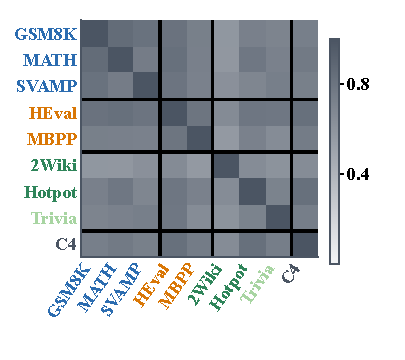
\includegraphics[width=\linewidth]{figs/v9_blocks_Qwen-Qwen3-1.7B_a.pdf}\subcaption{Raw Fisher cosine}\end{subfigure}
\hfill
\begin{subfigure}[t]{2.7in}\centering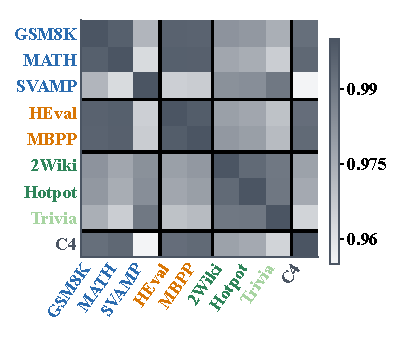
\includegraphics[width=\linewidth]{figs/v9_blocks_Qwen-Qwen3-1.7B_b.pdf}\subcaption{Log-Fisher cosine}\end{subfigure}
\\[3pt]
\begin{subfigure}[t]{2.7in}\centering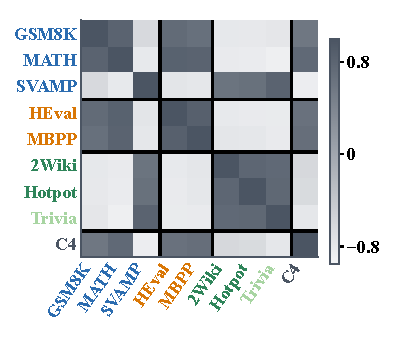
\includegraphics[width=\linewidth]{figs/v9_blocks_Qwen-Qwen3-1.7B_c.pdf}\subcaption{Residual log-Fisher cosine}\end{subfigure}
\hfill
\begin{subfigure}[t]{2.7in}\centering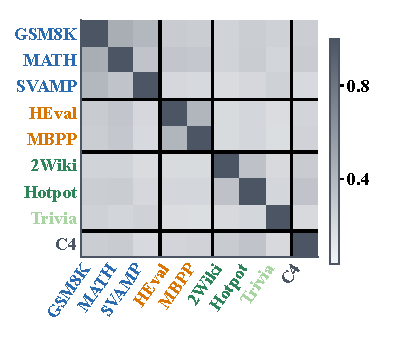
\includegraphics[width=\linewidth]{figs/v9_blocks_Qwen-Qwen3-1.7B_d.pdf}\subcaption{Top-0.1\% Jaccard}\end{subfigure}
\caption{Capability regions in gradient space for Qwen3-1.7B: pairwise similarity of per-benchmark gradient signatures under four metrics (raw Fisher cosine, log-Fisher cosine, shared-component-removed log-Fisher cosine, top-0.1\% coordinate Jaccard). Black lines separate the math, code, QA, and control blocks.}
\label{fig:blocks_Qwen_Qwen3_17B}
\end{figure}

\begin{figure}[p]
\centering

\includegraphics[width=5.5in]{figs/v9_blocks_Qwen-Qwen3-4B_legend.pdf}\\[1pt]
\begin{subfigure}[t]{2.7in}\centering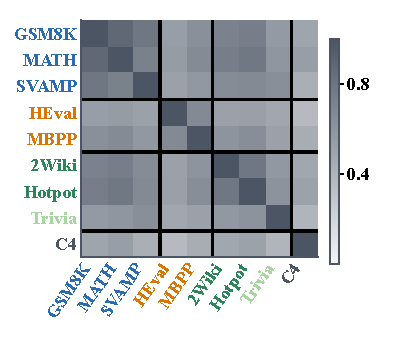
\includegraphics[width=\linewidth]{figs/v9_blocks_Qwen-Qwen3-4B_a.pdf}\subcaption{Raw Fisher cosine}\end{subfigure}
\hfill
\begin{subfigure}[t]{2.7in}\centering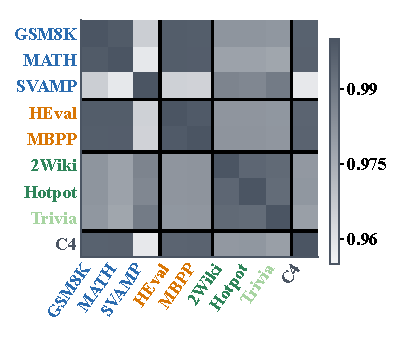
\includegraphics[width=\linewidth]{figs/v9_blocks_Qwen-Qwen3-4B_b.pdf}\subcaption{Log-Fisher cosine}\end{subfigure}
\\[3pt]
\begin{subfigure}[t]{2.7in}\centering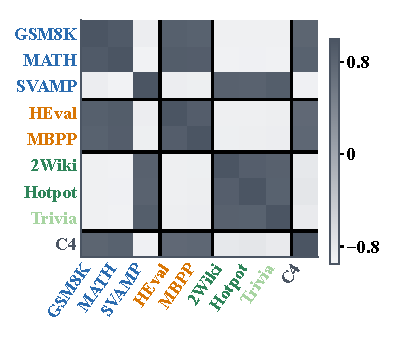
\includegraphics[width=\linewidth]{figs/v9_blocks_Qwen-Qwen3-4B_c.pdf}\subcaption{Residual log-Fisher cosine}\end{subfigure}
\hfill
\begin{subfigure}[t]{2.7in}\centering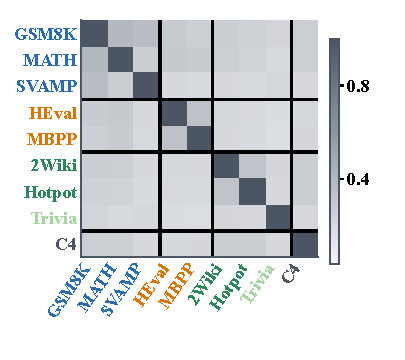
\includegraphics[width=\linewidth]{figs/v9_blocks_Qwen-Qwen3-4B_d.pdf}\subcaption{Top-0.1\% Jaccard}\end{subfigure}
\caption{Capability regions in gradient space for Qwen3-4B: pairwise similarity of per-benchmark gradient signatures under four metrics (raw Fisher cosine, log-Fisher cosine, shared-component-removed log-Fisher cosine, top-0.1\% coordinate Jaccard). Black lines separate the math, code, QA, and control blocks.}
\label{fig:blocks_Qwen_Qwen3_4B}
\end{figure}

\begin{figure}[p]
\centering

\includegraphics[width=5.5in]{figs/v9_blocks_gemma3-12b_legend.pdf}\\[1pt]
\begin{subfigure}[t]{2.7in}\centering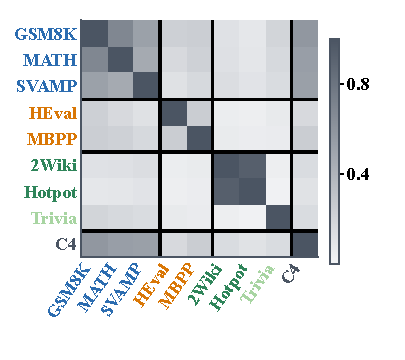
\includegraphics[width=\linewidth]{figs/v9_blocks_gemma3-12b_a.pdf}\subcaption{Raw Fisher cosine}\end{subfigure}
\hfill
\begin{subfigure}[t]{2.7in}\centering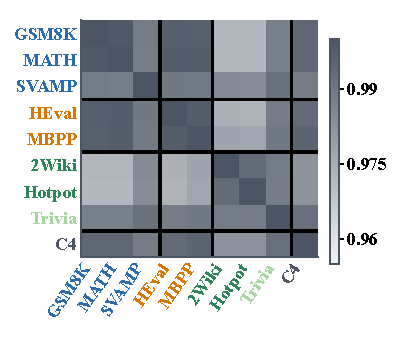
\includegraphics[width=\linewidth]{figs/v9_blocks_gemma3-12b_b.pdf}\subcaption{Log-Fisher cosine}\end{subfigure}
\\[3pt]
\begin{subfigure}[t]{2.7in}\centering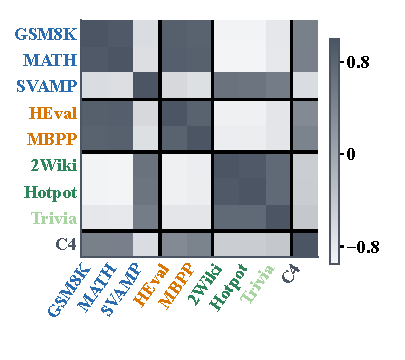
\includegraphics[width=\linewidth]{figs/v9_blocks_gemma3-12b_c.pdf}\subcaption{Residual log-Fisher cosine}\end{subfigure}
\hfill
\begin{subfigure}[t]{2.7in}\centering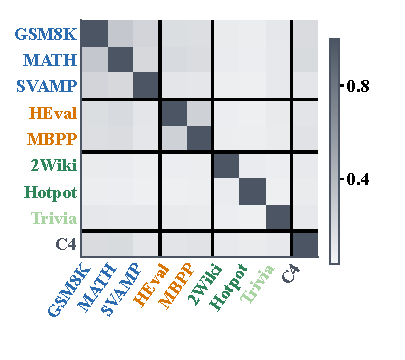
\includegraphics[width=\linewidth]{figs/v9_blocks_gemma3-12b_d.pdf}\subcaption{Top-0.1\% Jaccard}\end{subfigure}
\caption{Capability regions in gradient space for Gemma3-12B: pairwise similarity of per-benchmark gradient signatures under four metrics (raw Fisher cosine, log-Fisher cosine, shared-component-removed log-Fisher cosine, top-0.1\% coordinate Jaccard). Black lines separate the math, code, QA, and control blocks.}
\label{fig:blocks_gemma3_12b}
\end{figure}

\begin{figure}[p]
\centering

\includegraphics[width=5.5in]{figs/v9_blocks_gemma3-1b_legend.pdf}\\[1pt]
\begin{subfigure}[t]{2.7in}\centering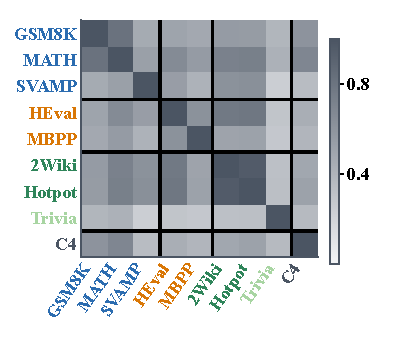
\includegraphics[width=\linewidth]{figs/v9_blocks_gemma3-1b_a.pdf}\subcaption{Raw Fisher cosine}\end{subfigure}
\hfill
\begin{subfigure}[t]{2.7in}\centering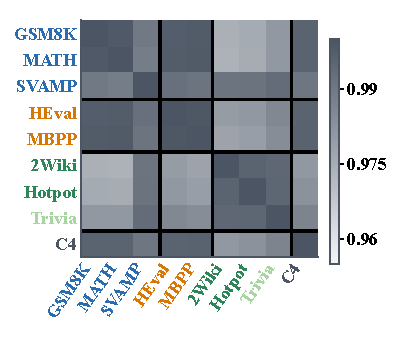
\includegraphics[width=\linewidth]{figs/v9_blocks_gemma3-1b_b.pdf}\subcaption{Log-Fisher cosine}\end{subfigure}
\\[3pt]
\begin{subfigure}[t]{2.7in}\centering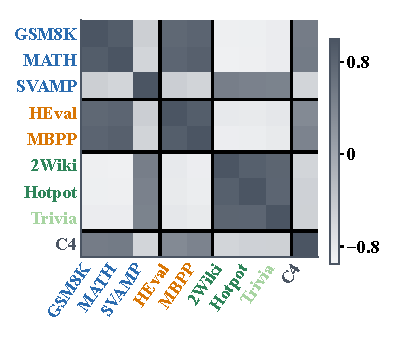
\includegraphics[width=\linewidth]{figs/v9_blocks_gemma3-1b_c.pdf}\subcaption{Residual log-Fisher cosine}\end{subfigure}
\hfill
\begin{subfigure}[t]{2.7in}\centering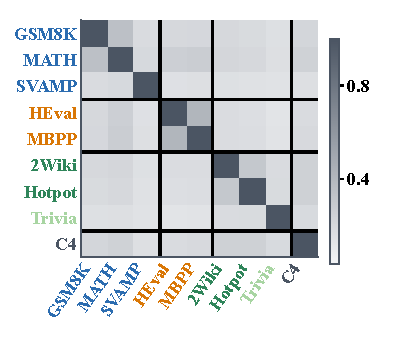
\includegraphics[width=\linewidth]{figs/v9_blocks_gemma3-1b_d.pdf}\subcaption{Top-0.1\% Jaccard}\end{subfigure}
\caption{Capability regions in gradient space for Gemma3-1B: pairwise similarity of per-benchmark gradient signatures under four metrics (raw Fisher cosine, log-Fisher cosine, shared-component-removed log-Fisher cosine, top-0.1\% coordinate Jaccard). Black lines separate the math, code, QA, and control blocks.}
\label{fig:blocks_gemma3_1b}
\end{figure}

\begin{figure}[p]
\centering

\includegraphics[width=5.5in]{figs/v9_blocks_gemma3-270m_legend.pdf}\\[1pt]
\begin{subfigure}[t]{2.7in}\centering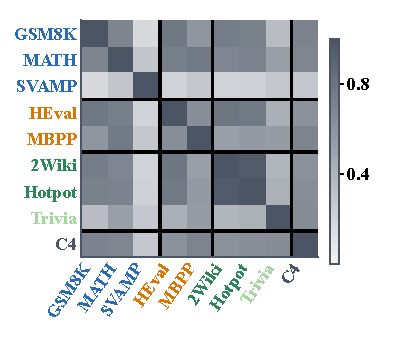
\includegraphics[width=\linewidth]{figs/v9_blocks_gemma3-270m_a.pdf}\subcaption{Raw Fisher cosine}\end{subfigure}
\hfill
\begin{subfigure}[t]{2.7in}\centering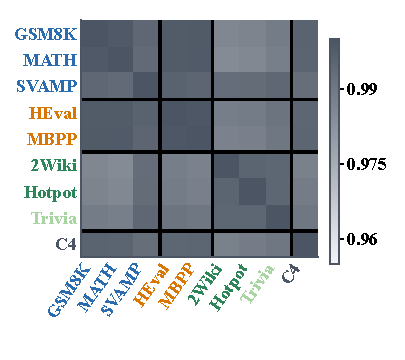
\includegraphics[width=\linewidth]{figs/v9_blocks_gemma3-270m_b.pdf}\subcaption{Log-Fisher cosine}\end{subfigure}
\\[3pt]
\begin{subfigure}[t]{2.7in}\centering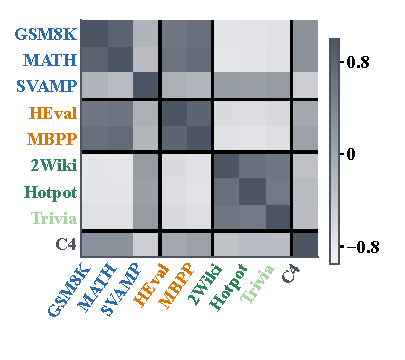
\includegraphics[width=\linewidth]{figs/v9_blocks_gemma3-270m_c.pdf}\subcaption{Residual log-Fisher cosine}\end{subfigure}
\hfill
\begin{subfigure}[t]{2.7in}\centering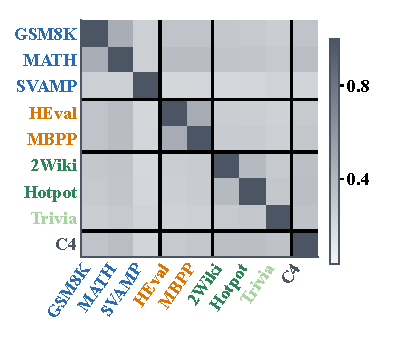
\includegraphics[width=\linewidth]{figs/v9_blocks_gemma3-270m_d.pdf}\subcaption{Top-0.1\% Jaccard}\end{subfigure}
\caption{Capability regions in gradient space for Gemma3-270M: pairwise similarity of per-benchmark gradient signatures under four metrics (raw Fisher cosine, log-Fisher cosine, shared-component-removed log-Fisher cosine, top-0.1\% coordinate Jaccard). Black lines separate the math, code, QA, and control blocks.}
\label{fig:blocks_gemma3_270m}
\end{figure}

\begin{figure}[p]
\centering

\includegraphics[width=5.5in]{figs/v9_blocks_gemma3-4b_legend.pdf}\\[1pt]
\begin{subfigure}[t]{2.7in}\centering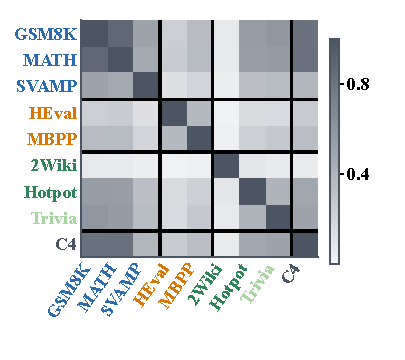
\includegraphics[width=\linewidth]{figs/v9_blocks_gemma3-4b_a.pdf}\subcaption{Raw Fisher cosine}\end{subfigure}
\hfill
\begin{subfigure}[t]{2.7in}\centering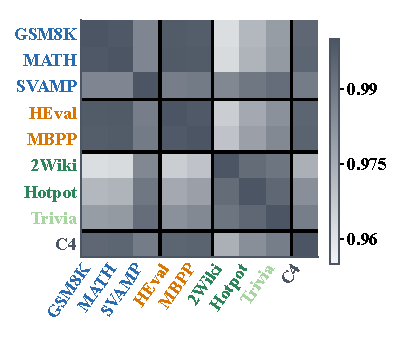
\includegraphics[width=\linewidth]{figs/v9_blocks_gemma3-4b_b.pdf}\subcaption{Log-Fisher cosine}\end{subfigure}
\\[3pt]
\begin{subfigure}[t]{2.7in}\centering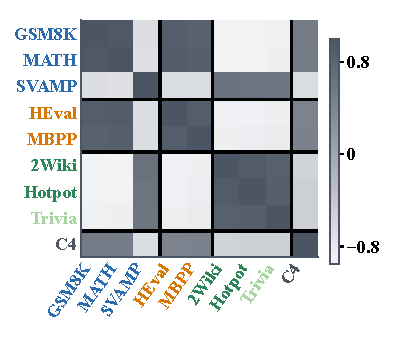
\includegraphics[width=\linewidth]{figs/v9_blocks_gemma3-4b_c.pdf}\subcaption{Residual log-Fisher cosine}\end{subfigure}
\hfill
\begin{subfigure}[t]{2.7in}\centering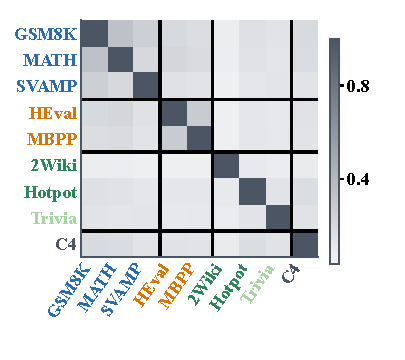
\includegraphics[width=\linewidth]{figs/v9_blocks_gemma3-4b_d.pdf}\subcaption{Top-0.1\% Jaccard}\end{subfigure}
\caption{Capability regions in gradient space for Gemma3-4B: pairwise similarity of per-benchmark gradient signatures under four metrics (raw Fisher cosine, log-Fisher cosine, shared-component-removed log-Fisher cosine, top-0.1\% coordinate Jaccard). Black lines separate the math, code, QA, and control blocks.}
\label{fig:blocks_gemma3_4b}
\end{figure}

\begin{figure}[p]
\centering

\includegraphics[width=5.5in]{figs/v9_blocks_gemma4-31b_legend.pdf}\\[1pt]
\begin{subfigure}[t]{2.7in}\centering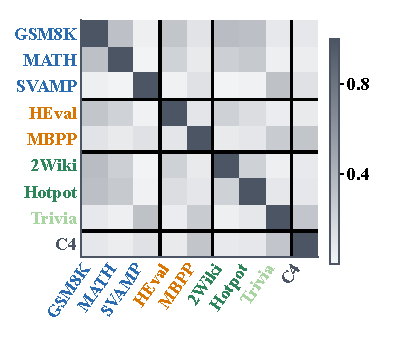
\includegraphics[width=\linewidth]{figs/v9_blocks_gemma4-31b_a.pdf}\subcaption{Raw Fisher cosine}\end{subfigure}
\hfill
\begin{subfigure}[t]{2.7in}\centering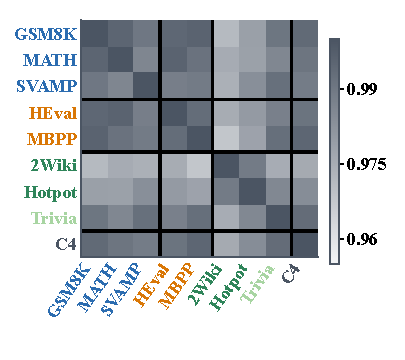
\includegraphics[width=\linewidth]{figs/v9_blocks_gemma4-31b_b.pdf}\subcaption{Log-Fisher cosine}\end{subfigure}
\\[3pt]
\begin{subfigure}[t]{2.7in}\centering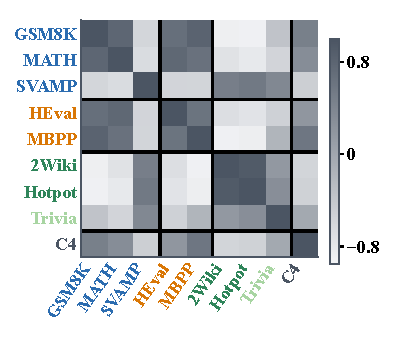
\includegraphics[width=\linewidth]{figs/v9_blocks_gemma4-31b_c.pdf}\subcaption{Residual log-Fisher cosine}\end{subfigure}
\hfill
\begin{subfigure}[t]{2.7in}\centering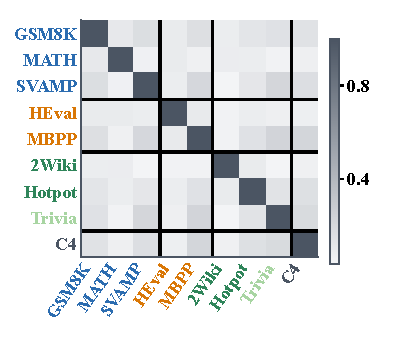
\includegraphics[width=\linewidth]{figs/v9_blocks_gemma4-31b_d.pdf}\subcaption{Top-0.1\% Jaccard}\end{subfigure}
\caption{Capability regions in gradient space for Gemma4-31B: pairwise similarity of per-benchmark gradient signatures under four metrics (raw Fisher cosine, log-Fisher cosine, shared-component-removed log-Fisher cosine, top-0.1\% coordinate Jaccard). Black lines separate the math, code, QA, and control blocks.}
\label{fig:blocks_gemma4_31b}
\end{figure}

\begin{figure}[p]
\centering

\includegraphics[width=5.5in]{figs/v9_blocks_muse-30b_legend.pdf}\\[1pt]
\begin{subfigure}[t]{2.7in}\centering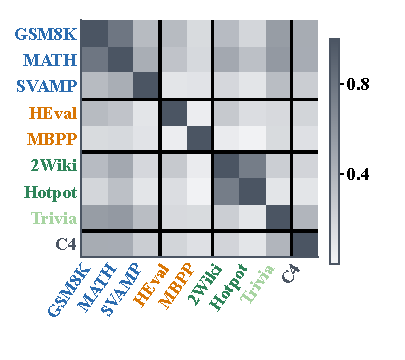
\includegraphics[width=\linewidth]{figs/v9_blocks_muse-30b_a.pdf}\subcaption{Raw Fisher cosine}\end{subfigure}
\hfill
\begin{subfigure}[t]{2.7in}\centering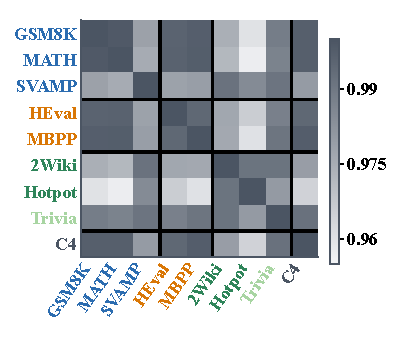
\includegraphics[width=\linewidth]{figs/v9_blocks_muse-30b_b.pdf}\subcaption{Log-Fisher cosine}\end{subfigure}
\\[3pt]
\begin{subfigure}[t]{2.7in}\centering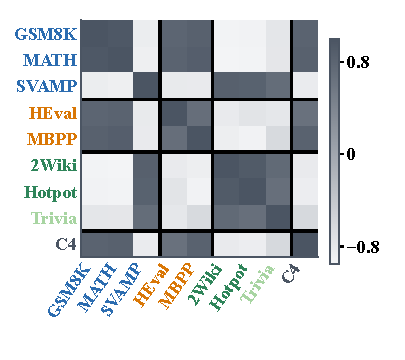
\includegraphics[width=\linewidth]{figs/v9_blocks_muse-30b_c.pdf}\subcaption{Residual log-Fisher cosine}\end{subfigure}
\hfill
\begin{subfigure}[t]{2.7in}\centering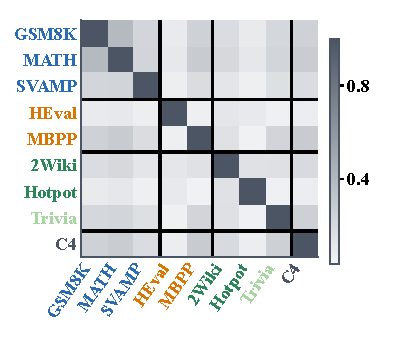
\includegraphics[width=\linewidth]{figs/v9_blocks_muse-30b_d.pdf}\subcaption{Top-0.1\% Jaccard}\end{subfigure}
\caption{Capability regions in gradient space for Muse-30B: pairwise similarity of per-benchmark gradient signatures under four metrics (raw Fisher cosine, log-Fisher cosine, shared-component-removed log-Fisher cosine, top-0.1\% coordinate Jaccard). Black lines separate the math, code, QA, and control blocks.}
\label{fig:blocks_muse_30b}
\end{figure}

\begin{figure}[p]
\centering

\includegraphics[width=5.5in]{figs/v9_blocks_olmo3-7b_legend.pdf}\\[1pt]
\begin{subfigure}[t]{2.7in}\centering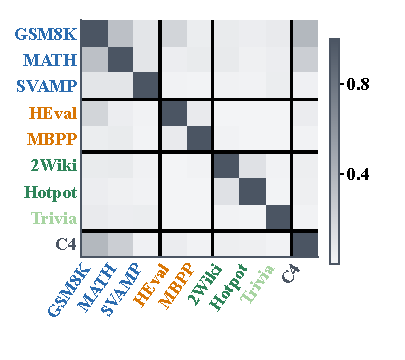
\includegraphics[width=\linewidth]{figs/v9_blocks_olmo3-7b_a.pdf}\subcaption{Raw Fisher cosine}\end{subfigure}
\hfill
\begin{subfigure}[t]{2.7in}\centering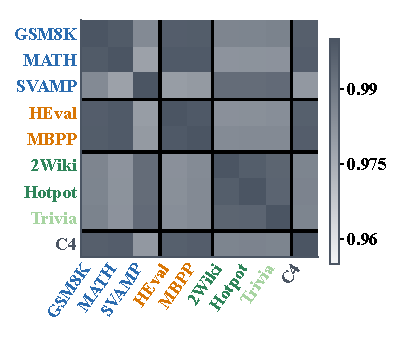
\includegraphics[width=\linewidth]{figs/v9_blocks_olmo3-7b_b.pdf}\subcaption{Log-Fisher cosine}\end{subfigure}
\\[3pt]
\begin{subfigure}[t]{2.7in}\centering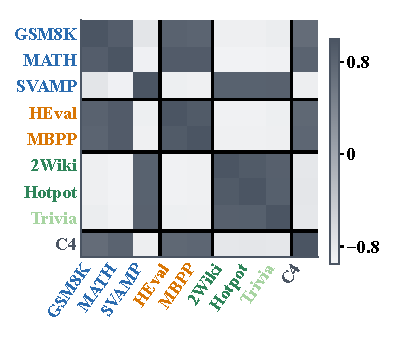
\includegraphics[width=\linewidth]{figs/v9_blocks_olmo3-7b_c.pdf}\subcaption{Residual log-Fisher cosine}\end{subfigure}
\hfill
\begin{subfigure}[t]{2.7in}\centering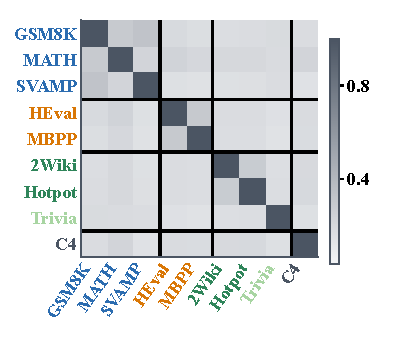
\includegraphics[width=\linewidth]{figs/v9_blocks_olmo3-7b_d.pdf}\subcaption{Top-0.1\% Jaccard}\end{subfigure}
\caption{Capability regions in gradient space for OLMo3-7B: pairwise similarity of per-benchmark gradient signatures under four metrics (raw Fisher cosine, log-Fisher cosine, shared-component-removed log-Fisher cosine, top-0.1\% coordinate Jaccard). Black lines separate the math, code, QA, and control blocks.}
\label{fig:blocks_olmo3_7b}
\end{figure}
